\documentclass[12pt,a4paper]{article}
\usepackage[utf8]{inputenc} 
\usepackage{latexsym,amssymb,amsmath}
%\usepackage{xltxtra} % charge aussi fontspec et xunicode,
                     % nécessaires...
% \usepackage[latin1]{inputenc}
\usepackage[T1]{fontenc}
\usepackage[francais]{babel}
\usepackage{hyperref}
\usepackage{listings} \lstset{language=C, showstringspaces=false}

\topmargin -1cm 
\oddsidemargin -10mm 
%\evensidemargin 0mm 
\textheight 27cm 
\textwidth 18cm 
\columnsep 4.1mm

\parindent 1.0em 
\headsep 0mm 
\headheight 0pt 
\lineskip 0pt
\parskip 1em

\normallineskip 0pt 
\def\baselinestretch{1}

\sloppy \hbadness=10000

%%%% PACKAGES
\usepackage[scale=0.74,vmargin=1.4cm ]{geometry}

\usepackage{latexsym,amssymb,amsmath}
\usepackage[utf8]{inputenc}
\usepackage[T1]{fontenc}
\usepackage[francais]{babel}
\usepackage{textcomp} %pour euro
\usepackage{ifpdf}
\ifpdf
\usepackage[pdftex]{graphicx}
\else
\usepackage[dvips]{graphicx}
\usepackage{pstricks, pst-tree, pst-node}
\fi 
\usepackage{calc}
\usepackage{moreverb}
\usepackage{version}
\usepackage{url}
\usepackage{multicol}
\usepackage{listings}
\usepackage{tikz}
\usetikzlibrary{shapes,arrows}
\usepackage{rotating}
\usepackage{subfigure}

\lstset{language=C, showstringspaces=false}
\usepackage{enumerate}

%%%% COMMANDES
\newcommand{\entete}[1]{%
\noindent
\rule{\linewidth}{0.5mm}\\
\noindent
Universit\'e Paris-Nord \hfill Ann\'ee 2012-2013\\
\noindent
Algorithmique et programmation \hfill DUT R\&T 1\\
\rule{\linewidth}{0.5mm}
\begin{center}
\Large\bf #1
\end{center}
\vspace{0.5cm}
}

\newcommand{\C}[1]{{\upshape\texttt{#1}}}
\newenvironment{correction}{\paragraph{Correction.}\hrulefill\begin{itshape}}{\end{itshape}\hrulefill}
\newenvironment{cpii}{}{} % pour les liens spécifiques au CP2I
\excludeversion{cpii}
\newenvironment{baremeenv}{\paragraph{Barème.} \begin{itshape}}{\end{itshape}}
%\excludeversion{baremeenv}

% Hack tres moche pour des enumerate qui continuent la numérotation...
% j'ai deja fait ca ailleurs et mieux mais ou ?
\newcounter{saveenumi}
\newenvironment{newenu}
{\begin{enumerate}}
{\setcounter{saveenumi}{\value{enumi}}\end{enumerate}}
\newenvironment{lastenu}
{\begin{enumerate}\setcounter{enumi}{\value{saveenumi}}}
{\setcounter{saveenumi}{\value{enumi}}\end{enumerate}}

\newcommand{\bbbn}{\ensuremath{\mathbb{N}}}
\newcommand{\bbbr}{\ensuremath{\mathbb{R}}}

\newcommand{\carriagereturn}{\C{$\backslash$n}}
%%% Local Variables: 
%%% mode: latex
%%% TeX-master: t
%%% End: 

%\excludeversion{cpii}

\begin{document}
\entete{TP ddd}

\newcommand{\puis}{\ensuremath{\rightarrow\ }}

\section{Déboguer un programme avec ddd}

Un débogueur permet avant tout de suivre pas-à-pas l'exécution d'un
programme, tout en permettant de visualiser les valeurs des variables
de ce programme. Il est surtout utile pour trouver les erreurs
présentes dans le programme (quand celui-ci se compile correctement,
mais ne fait pas ce qu'on pense qu'il devrait faire). 

Le débogueur le plus répandu sous Linux est {\bf \tt gdb}. Il fonctionne
en ligne de commande, sous une forme uniquement textuelle, qui plaît à
certains mais peut sembler difficile à maîtriser. Il existe également de
nombreux débogueurs graphiques, qui en général ne sont que des
frontends de {\tt gdb}.

L'objectif de ce TP est de commencer à vous familiariser avec le
débogueur {\tt \bf ddd}, \emph{the Data Display Debugger}, dont vous
trouverez par ailleurs de nombreux didacticiels en cherchant {\tt ddd}
dans Google !


Pour cette initiation, commencez par entrer le programme suivant, qui
calcule la somme des carrés des $n$ premiers entiers positifs~: entrez
ce programme dans un éditeur de texte, et sauvegardez-le sous le nom
{\tt sommeCarres.c}~!

\lstinputlisting{sommeCarres.c}


\begin{cpii}
  Programme accessible à l'adresse~:\\
  \href{https://webcours.ig-edu.univ-paris13.fr/mod/resource/view.php?id=479}{https://webcours.ig-edu.univ-paris13.fr/mod/resource/view.php?id=479}.
\end{cpii}

\subsection{Compilation et exécution}

Dans une console, placez-vous dans
le répertoire qui contient {\tt sommeCarres.c}, et tapez la commande~:
\begin{verbatim}
gcc sommeCarres.c -o sommeCarres
\end{verbatim}

Si \texttt{gcc} rapporte des erreurs dans le programme, corrigez-les,
puis relancez la commande jusqu'à ce qu'il n'y en ait plus.

Lancez ensuite le programme en tapant la commande~:
\begin{verbatim}
./sommeCarres
\end{verbatim}

Entrez un entier. Trouvez-vous le résultat normal~?

\subsection{Compilation et déboguage}

Pour pouvoir déboguer un programme en C, il faut le compiler avec
l'{\bf option \tt -g} de {\tt gcc}. Dans une console, placez-vous dans
le répertoire qui contient {\tt sommeCarres.c}, et tapez la commande~:
\begin{verbatim}
gcc -g sommeCarres.c -o sommeCarres
\end{verbatim}


\subsection{Exécution du programme dans le débogueur}

Après avoir compilé votre programme, lancez le débogueur en tapant la
commande {\bf \tt ddd}~!

Pour ouvrir le programme à déboguer, passez par le menu ``File \puis
Open Program...'', sélectionnez le répertoire de votre programme dans
la partie gauche, puis {\tt sommeCarres} dans la partie droite, et
cliquez sur ``Open''.


\begin{center}
  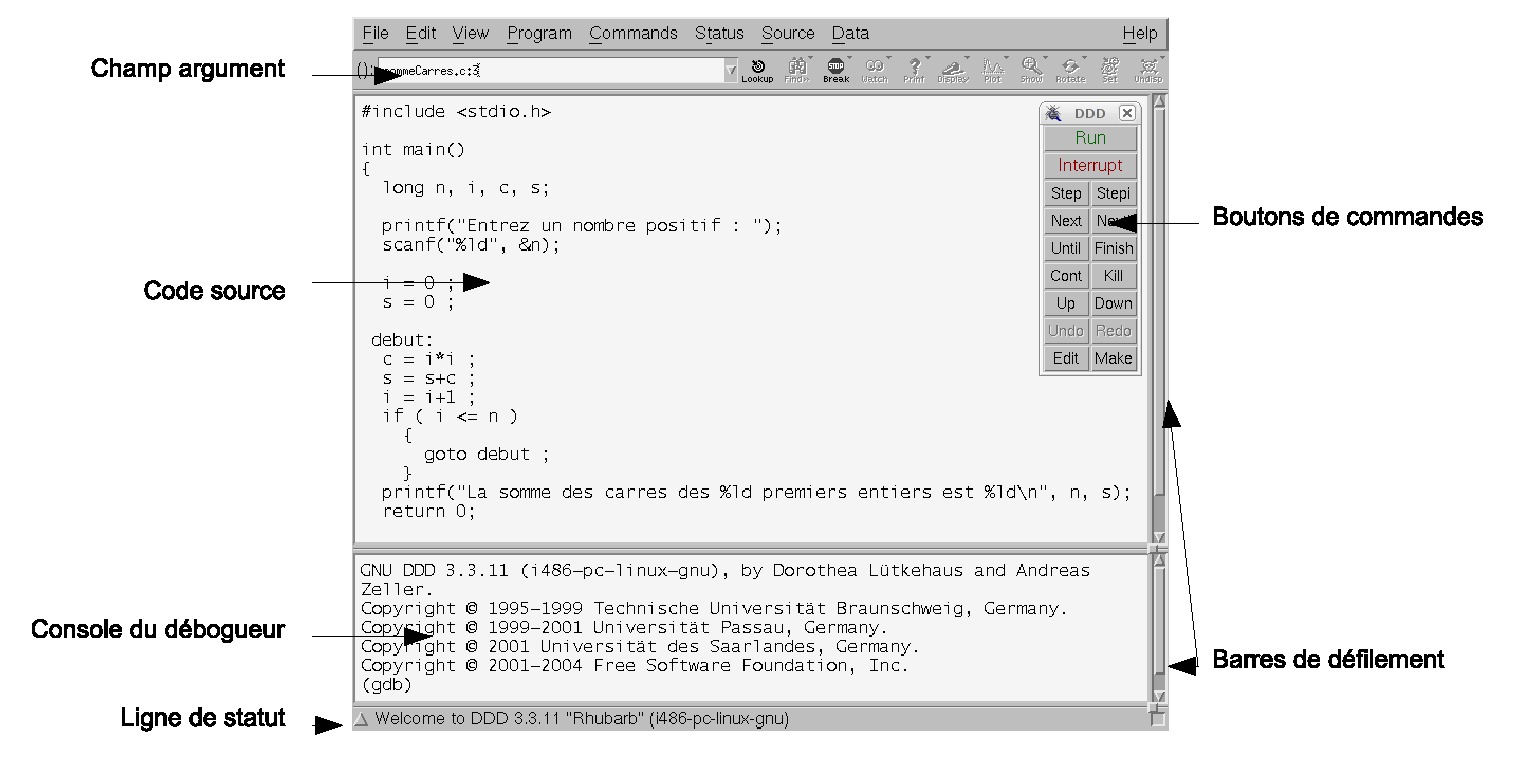
\includegraphics[width=\linewidth]{ddd2.eps}
\end{center}



Le {\bf code source} du programme à déboguer apparaît au centre de la
fenêtre; vous pouvez utiliser la barre de défilement pour vous
promener dans ce fichier.

\bigskip

La {\bf console de déboguage} contient de l'information sur la version
de DDD, ainsi que l’« invite de commandes » de GDB. 
\begin{verbatim}
GNU DDD 3.3.11 (i486-pc-linux-gnu), by Dorothea Lütkehaus and Andreas Zeller.
Copyright © 1995-1999 Technische Universität Braunschweig, Germany.
Copyright © 1999-2001 Universität Passau, Germany.
Copyright © 2001 Universität des Saarlandes, Germany.
Copyright © 2001-2004 Free Software Foundation, Inc.
(gdb)
\end{verbatim}
On peut
interagir directement avec GDB en tapant des commandes dans cette
console, comme on peut également utiliser les {\bf boutons de
  commande} ou les menus de {\tt ddd}.


\bigskip



La première chose à faire est de lancer le programme, en cliquant sur
le bouton de commande {\bf Run}, ou en tapant ``r'' suivi de la
touche ``Entrée'' dans la console de déboguage. Les entrées et sorties
du programme se déroulent dans la fenêtre de déboguage~: le programme
demande d'entrer un nombre positif, puis affiche le résultat du
calcul~:

\begin{verbatim}
(gdb) r
Entrez un nombre positif : 4
La somme des carres des 4 premiers entiers est 10

Program exited normally.
\end{verbatim}

Gdb affiche gentiment que le programme s'est arrêté normalement,
car il a renvoyé la valeur $0$ (\textit{EXIT\_SUCCESS}) en retour. Si
la dernière ligne du code
source était ``{\tt return 1;}'', gdb afficherait le message~:

\begin{verbatim}
Program exited with code 01.
\end{verbatim}

Toutes les valeurs de retour du programme différentes de 0 sont
considérées comme des codes d'erreur.

\bigskip

Les entrées-sorties du programme peuvent aussi se faire dans une
fenêtre séparée, de manière à réserver la console de déboguage aux
messages de gdb. Pour cela, activez le menu {\tt View \puis Execution
  Window}, puis relancez le programme~!


\subsection{Exécution pas-à-pas}

Pour observer maintenant de plus près le déroulement du programme,
il faut placer un point d’arrêt (ou \emph{breakpoint}), qui fera s’
arrêter {\tt sommeCarres} à l’endroit qui nous intéresse. Cliquez
dans l’espace blanc à 
gauche de l’initialisation de $s$. Le champ argument (): contient
maintenant la position (sommeCarre.c:11). Maintenant, cliquez sur {\tt
  Break} pour créer un point d’arrêt à cet emplacement. Vous voyez un
petit signal stop rouge apparaître dans la ligne 10. 

\bigskip

Relancez ensuite le programme comme précédemment, et entrez le nombre
$4$.


L'exécution stoppe au bout d'un instant, lorsque le point d'arrêt
est atteint. Cela est signalé dans la console de déboguage~:

\begin{verbatim}
Breakpoint 1, main () at sommeCarres.c:11
\end{verbatim}

La ligne couramment exécutée (en réalité, la ligne qui va être
exécutée) est indiquée par une flèche verte~:

$\Rightarrow$ \lstinline{s = 0 ;}

\bigskip

Vous pouvez maintenant examiner les valeurs des variables. Pour
examiner une variable simple, il suffit de placer le pointeur de la
souris sur son nom et le laisser dessus. Au bout d’une seconde, une
petite fenêtre surgit montrant avec la valeur de la variable. Essayez
avec la variable $n$ pour voir sa valeur ($4$). Les autres variables
(\textit{s}, \textit{i} et \textit{c}) ne sont pas initialisées et
vous verrez probablement des valeurs
fantaisistes si vous pointez dessus.


Pour exécuter la ligne courante, cliquez sur le bouton de commande
{\bf Next}. La flèche avance sur la ligne suivante. Maintenant,
pointez de nouveau sur $s$ pour voir que la valeur a changé et que cette
variable a bien été initialisée à $0$.

Continuez à appuyer sur Next, jusqu'à atteindre la ligne du
\emph{<<~i = i + 1 ;~>>}. On est arrivé à la fin du bloc d'instruction
de la boucle \textit{for}. Appuyez à nouveau sur Next, et le pointeur
retourne sur la ligne du \textit{for}.

Examinez les valeurs des variables $i$ et
$n$ : la condition $i<n$ étant vraie, le prochain apppui sur Next fera
entrer le pointeur d'exécution dans la boucle (comme la première
fois). Continuez ainsi jusqu'à ce que le programme se termine~!

Vous pouvez aussi utiliser le bouton {\bf Until} pour forcer le
programme à s'exécuter jusqu'à ce que la ligne suivante soit
atteinte~: relancez le programme, et lorsque la flèche verte est sur
la ligne du \textit{<<~for~>>}, cliquez sur \textit{Until}. La
première fois, l'exécution se poursuit comme avec le bouton
\textit{Next}, mais la seconde fois où vous passez sur le
\textit{<<~for~>>}, si vous cliquez sur \textit{Until}, le
programme continuera à s'exécuter
sans s'arrêter jusqu'à atteindre la ligne du \emph{printf}. Vous
pouvez vérifier qu'il a effectivement effectué les
instructions de la boucle en observant le contenu des variables $s$,
$c$ et $i$ avant et après avoir appuyé sur \textit{Until}.

Pourquoi cette différence de comportement entre les deux appuis sur
\textit{Until}~? Simplement parce que les termes \textit{ligne
  suivante} désignent en fait l'instruction suivante dans le programme
\textbf{compilé}. La ligne du \textit{for} a été traduite par le
compilateur en  une série d'instructions machine, dont certaines se
trouvent avant le corps de la boucle, et d'autres en fin de
boucle. Vous pouvez voir le code machine correspondant au point
d'exécution en utilisant le menu \textbf{View $\Rightarrow$ Machine Code
  Window}. En déroulant le programme, vous pouvez constater que le
premier arrêt sur la ligne du \textit{for} correspond à la ligne
\verb|<main+55>| du code machine (c'est le début de la boucle dans le
programme compilé, qui correspond à l'initialisation de $i$ à $1$),
alors que les arrêts suivants sur la ligne du
\textit{for} correspondent à la ligne \verb|<main+84>| du code machine
(c'est la fin de la boucle dans le programme compilé, et l'instruction
machine correspond à l'incrémentation de $i$).

Pour bien voir la différence entre le code source et le code compilé,
vous pouvez exécuter le programme en utilisant le bouton
\textit{Nexti} au lieu de \textit{Next}~: le programme s'arrête à la
prochaine instruction machine, plutôt qu'à la prochaine instruction
dans le code source. Vous pouvez constater par exemple qu'il faut
plusieurs instructions machine pour l'affectation \textit{<<~c =
  i*i~;~>>}, alors qu'il n'en faut qu'une seule pour \textit{<<~i =
  i+1~;~>>}. 




\subsection{Examen des variables}


Laisser le pointeur traîner au-dessus du nom d'une variable n'est pas
le seul moyen de l'examiner. Vous pouvez également utiliser les
commandes à côté du champ argument~(): cliquez sur une variable afin de
la faire apparaître dans le champ argument~(), puis cliquez sur le
bouton {\tt Print} (il faut que le programme soit lancé et arrêté sur
un point d'arrêt)~: la valeur s'affiche sur la console de déboguage.

Si vous maintenez le bouton {\tt Print} enfoncé pendant plus d'une
seconde, un menu apparaît. Déplacez alors la souris sur les
différentes options, et une explication s'affiche dans la barre de
statut. Relâchez la souris sur {\tt Whatis()}, et la console affiche
le type de la variable ({\tt int}).

Les commandes {\tt Print} n'agissent qu'une fois~: il faut cliquer
dessus à chaque fois que l'on veut un renseignement sur une
variable. En revanche, la bouton {\tt Display}
permet d'observer la variable du champ argument de façon
permanente. Lorsque vous l'utilisez, vous voyez apparaître la variable
observée dans une nouvelle sous-fenêtre, avec sa valeur. Vous pouvez
répéter l'opération avec plusieurs variables, qui vont apparaître les
unes au-dessous des autres. Utilisez la barre de défilement pour les
examiner. Vous pouvez également réorganiser leur disposition par des
glisser-déposer pour en avoir une meilleure vue. Déroulez ensuite le
programme pas-à-pas~: vous pouvez observer les valeurs des variables
qui se modifient à chaque instruction. Lorsqu'une valeur vient
d'être modifiée par une instruction, elle apparaît sur fond jaune.


Vous pouvez obtenir une vue compacte de plusieurs variables de la
façon suivante~: sélectionnez les cadres des variables que vous voulez
regrouper, en maintenant la touche \textit{Shift} (appelée aussi
\textit{Maj.} et représentée par une flèche vers le haut) enfoncée
pendant que
vous cliquez sur les cadres~; ensuite, utilisez le bouton {\tt Undisp
  \puis Cluster()}, ce qui les fait apparaître dans un unique cadre
nommé {\tt Displays}. Pour réaliser l'opération inverse, sélectionnez
le cadre {\tt Displays}, et utilisez {\tt Undisp \puis Uncluster()}.

Pour supprimer l'affichage d'un cadre dans cette fenêtre,
sélectionnez le cadre, et cliquez simplement sur {\tt Undisp}.


Vous pouvez également modifier la valeur d'une variable
en la faisant apparaître dans le champ argument () puis en cliquant
sur le bouton {\tt Set}.


\subsection{à l'action !}

Affichez dans le cadre \texttt{Displays} un cluster contenant toutes
les variables du programme. 

Examinez particulièrement le contenu de la variable $i$ au second
passage sur la ligne \textit{c = i*i ;}. Cela doit vous mettre sur la
piste d'une première erreur. Corrigez cette erreur et recompilez le
programme avant de le relancer dans le débogueur.

Le résultat devrait toujours être faux. Pour voir d'où vient l'erreur,
déroulez à nouveau le programme en vous concentrant sur le dernier
passage dans la boucle. Corrigez, recompilez, relancez~!

Finalement, lorsque vous entrez $0$ comme valeur de $n$, le résultat
devrait être faux. Cherchez pourquoi, corrigez, recompilez, relancez~!



% \subsection{pile d'appels de fonctions}

% Le programme suivant effectue le même travail que le précédent, mais
% le calcul des carrés est délégué à une fonction {\tt calcul}.


% \lstinputlisting{sommeCarres2.c}


% \begin{cpii}
%   Programme accessible à l'adresse~:\\
%   \href{https://webcours.ig-edu.univ-paris13.fr/file.php/37/Travaux_pratiques/TP_deboguage/sommeCarres2.c}{https://webcours.ig-edu.univ-paris13.fr/file.php/37/Travaux\_pratiques/TP\_deboguage}/\\
%     \href{https://webcours.ig-edu.univ-paris13.fr/file.php/37/Travaux_pratiques/TP_deboguage/sommeCarres2.c}{sommeCarres2.c}.
% \end{cpii}


% Après l'avoir compilé et chargé dans {\tt ddd}, placez un point
% d'arrêt sur la ligne \lstinline{c = calcul(n);} et lancez-le. Lorsque
% le point d'arrêt est atteint, affichez les variables $n$ et $s$ dans
% la fenêtre {\tt Display}. $n$ contient la valeur que vous avez
% entrée, et $s$, qui n'a pas été initialisée, contient une valeur
% aléatoire. Essayez de faire afficher les variables $limite$, $i$ ou
% $c$~: une erreur apparaît dans la console de déboguage, car ces
% variables n'existent pas dans le contexte de la fonction $main$.

% Utilisez ensuite le bouton {\tt Next} du panneau de commandes~:
% la fonction est exécutée, et la valeur de retour est affectée à $s$.

% Relancez le programme depuis le début (boutons {\tt Kill} puis {\tt
%   Run}) jusqu'au point d'arrêt, mais utilisez cette fois le bouton
% {\tt Step}~: celui-ci permet d'observer l'exécution de la fonction
% appelée ({\tt calcul}). Remarquez que lorsque le point d'exécution
% entre dans la fonction {\tt calcul}, les variables $n$ et $s$
% disparaissent de la fenêtre {\tt Display}. En revanche, vous pouvez
% maintenant y faire apparaître $limite$, $i$, $c$, et à nouveau $s$.

% Utilisez le menu {\tt Data \puis Dispays} pour voir la liste des
% variables observées. Vous voyez apparaître deux fois la variable $s$,
% mais avec une valeur différente dans la colonne $scope$
% (i.e. portée). Les variables affichées dans la fenêtre {\tt Display}
% sont celles dont la portée inclut le point d'exécution.

% Faites quelques pas d'exécution dans la fonction {\tt calcul}, puis
% utilisez le menu {\tt Status \puis Backtrace...}. La fenêtre qui
% apparaît vous montre la {\bf pile d'exécution}~: elle montre que la
% fonction $main$ est en attente à la ligne 25 et qu'elle a appelé la
% fonction $calcul$, qui est en attente là où vous l'avez laissée. Vous
% pouvez vous déplacer dans cette pile en cliquant sur la ligne qui vous
% intéresse, pour observer les valeurs des variables disponibles à un
% étage de la pile. Cliquez sur la ligne de $main$~: la fenêtre
% $Display$ affiche à nouveau les variables $n$ et $s$ de la fonction
% $main$, et vous pouvez remarquer que $s$ n'a pas la même valeur que le
% $s$ de l'étage $calcul$. Retournez à l'étage $calcul$, et utilisez le
% bouton de commande $Finish$, qui permet de continuer l'exécution de la
% fonction courante jusqu'à ce qu'elle se termine. L'exécution revient à
% la ligne \lstinline{c = calcul(n);} et vous remarquez que $c$ n'a
% toujours pas changé de valeur. En effet, cette ligne contient deux
% instruction~: l'appel à la fonction $calcul$, qui est terminé, puis
% l'affectation du résultat à la variable $c$, qui n'a pas encore été
% effectuée. Appuyez sur le bouton $Step$, et cette fois-ci, $c$ prend
% la valeur de retour de l'appel à $calcul(n)$.


% Pour jouer un peu avec cette pile d'exécution, lancez le programme
% suivant dans le débogueur, après avoir mis un point d'arrêt dans la
% fonction $calcul$ sur la ligne \lstinline{s=calcul(limite-1)}~:

% \lstinputlisting{sommeCarres3.c}

% \begin{cpii}
%   Programme accessible à l'adresse~:\\
%   \href{https://webcours.ig-edu.univ-paris13.fr/file.php/37/Travaux_pratiques/TP_deboguage/sommeCarres3.c}{https://webcours.ig-edu.univ-paris13.fr/file.php/37/Travaux\_pratiques/TP\_deboguage}/\\
%     \href{https://webcours.ig-edu.univ-paris13.fr/file.php/37/Travaux_pratiques/TP_deboguage/sommeCarres3.c}{sommeCarres3.c}.
% \end{cpii}

% Entrez la valeur 10 pour $n$, puis continuez l'exécution en utilisant
% le bouton de commande {\tt Cont}~: l'exécution du
% programme se poursuit jusqu'au prochain point d'arrêt. Affichez la
% fenêtre {\tt backtrace} et constatez qu'à chaque appui sur {\tt Cont},
% la pile d'exécution s'agrandit. En effet, la fonction {\tt calcul}
% s'appelle elle-même. En utilisant la fenêtre {\tt display} et en vous
% déplaçant dans la pile d'appel, vous pouvez observer qu'à chaque
% <<~étage~>> de la pile, les variables accessibles dans la fonction
% {\tt calcul} ont des valeurs différentes.




% \subsection{arguments et tableaux}

% Le programme suivant doit inverser une liste d'entiers passés en
% arguments. 

% \lstinputlisting{inverseListe.c}.

% \begin{cpii}
%   Programme accessible à l'adresse~:\\
%   \href{https://webcours.ig-edu.univ-paris13.fr/file.php/37/Travaux_pratiques/TP_deboguage/inverseListe.c}{https://webcours.ig-edu.univ-paris13.fr/file.php/37/Travaux\_pratiques/TP\_deboguage}/\\
%     \href{https://webcours.ig-edu.univ-paris13.fr/file.php/37/Travaux_pratiques/TP_deboguage/inverseListe.c}{inverseListe.c}.
% \end{cpii}

% Compilez-le sous le nom {\tt inverseListe}, puis lancez-le
% en ligne de commande~:

% \begin{verbatim}
% $ ./inverseListe 8000 7000 5000 1000 4000
% 135145 4000 1000 5000 7000 
% $
% \end{verbatim}
% On constate que la liste obtenue n'est pas exactement la bonne~: le
% premier élément semble fantaisiste, et le $8000$ a disparu. 

% Ouvrez le programme dans {\tt ddd} et placez un point d'arrêt sur  la
% ligne <<~\lstinline{a = (int *) malloc...}~>>. Lancez-le ensuite par
% le menu {\tt
% Program \puis Run...}. Sous {\tt Run with arguments}, entrez les arguments
% précédents~: 8000 7000 5000 1000 4000

% Lorsque le programme s'arrête, faites {\tt Next}. $a$ contient maintenant
% l'adresse d'un tableau d'entiers. Affichez la valeur du premier
% élément de $a$ en entrant {\tt a[0]} dans le champ argument et en
% cliquant sur le bouton {\tt Display}. Pour voir tous les membres de $a$
% en même temps, vous devez utiliser un opérateur spécial de
% GDB. Puisque $a$ a été alloué dynamiquement, GDB ne connaît pas sa
% taille ; vous devez explicitement utiliser l’opérateur @ pour
% indiquer une « tranche de tableau ». Saisissez a[0]@(argc - 1) dans le
% champ argument et cliquez sur le bouton Display. Le contenu de a est
% maintenant montré dans la fenêtre de données. Cliquez sur {\tt Rotate}
% pour faire tourner horizontalement le tableau.

% Arrive maintenant l’affectation des membres de $a$ :


% \begin{lstlisting}
%   for (i = 0; i < argc - 1; i++)
%     a[i] = atoi(argv[i + 1]);
% \end{lstlisting}

% Cliquez sur {\tt Next} plusieurs fois pour voir comment les membres
% individuels de $a$ sont affectés les uns après les autres.

% Lorsque vous arrivez sur l'appel à la fonction {\tt inverse},
% cliquez sur {\tt Next} à nouveau~: vous voyez que le problème est
% apparu dans le contenu de $a$.

% Relancez donc le programme. Cette fois vous allez sauter
% l'initialisation de a et vous rendre directement à l’appel de {\tt
%   inverse}. Effacez l'ancien point d'arrêt en le sélectionnant et en
% cliquant sur le bouton {\tt Clear}. Ensuite créez un nouveau point
% d'arrêt juste avant l'appel de {\tt inverse}. Pour exécuter le
% programme de nouveau, avec les mêmes arguments, sélectionnez {\tt
%   Program \puis Run Again}.

% Entrez cette fois dans la fonction {\tt inverse} en cliquant sur {\tt
%   Step}. Examinons si les arguments de {\tt inverse} sont
% corrects. Saisissez {\verb+a[0]@taille+} dans le champ arguments et
% cliquez sur le bouton {\tt Display}~: surprise ! Il y a une valeur
% supplémentaire à la fin du tableau. D'où vient cette valeur
% supplémentaire ? La réponse est simple : la taille du tableau passée à
% {\tt inverse} dans le paramètre {\tt taille} est trop grande de une
% unité. Le nombre supplémentaire est une valeur imprévisible qui se
% trouvait dans la mémoire à la suite de $a$. Mais cette valeur va être
% inversée avec les autres.

% Pour voir si tel est effectivement le problème, vous pouvez affecter à
% {\tt taille} la valeur correcte. Choisissez {\tt taille} dans le code
% source et cliquez sur {\tt Set}. Une boîte de dialogue apparaît dans
% laquelle vous pouvez changer la valeur de la variable. Donnez-lui la
% valeur $5$ puis cliquez sur OK. Ensuite, cliquez sur {\tt Cont} pour
% terminer le programme. Succès !

% Ayant trouvé la cause du problème vous pouvez maintenant corriger le
% code source. Remplacez la ligne 

% \begin{lstlisting}
%   inverse(a, argc);
% \end{lstlisting}
% par l’appel correct
% \begin{lstlisting}
%   inverse(a, argc - 1);
% \end{lstlisting}

% Recompilez, relancez, ça marche !



\begin{center}
  \noindent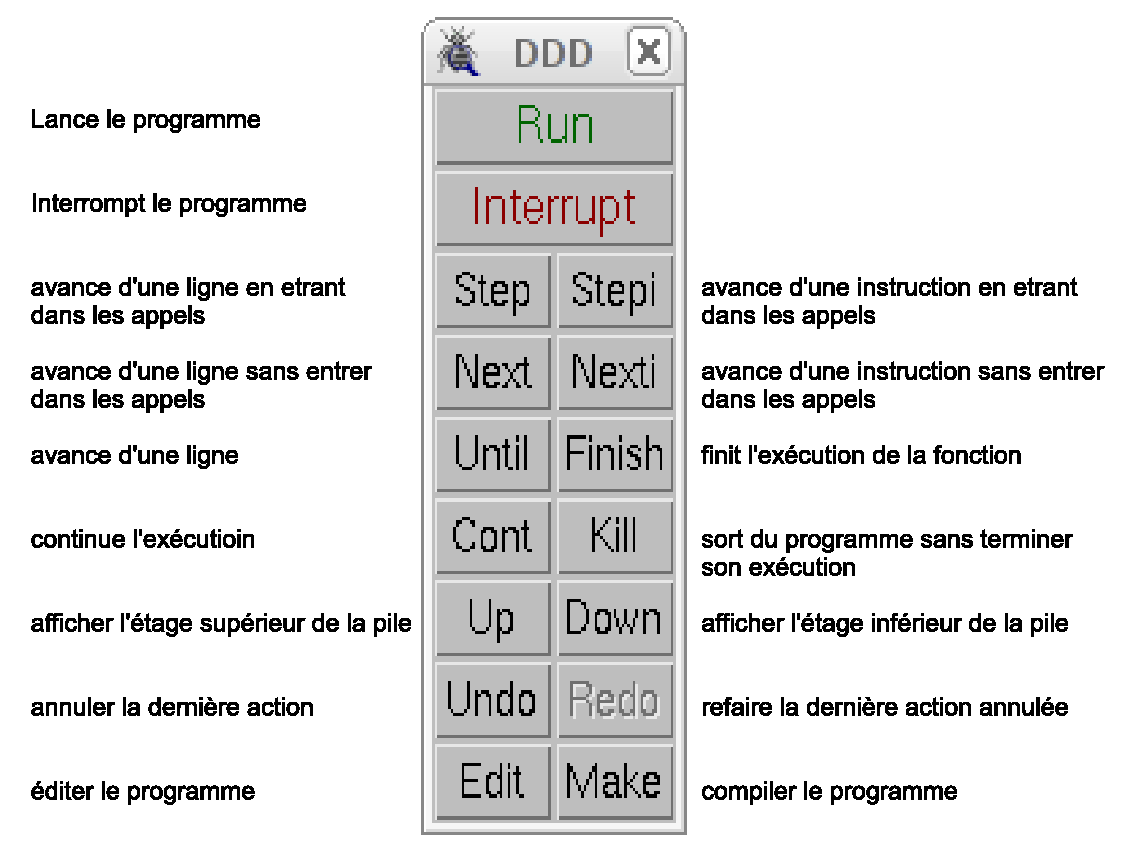
\includegraphics[width=\linewidth]{commandes.eps}
\end{center}
\end{document}
